\documentclass[a4paper, DIV11, abstracton]{scrartcl}
\usepackage{color,graphicx}			% graphics package

\usepackage{microtype}				% optical margin alignment
\usepackage[T1]{fontenc}			% umlauts for european languages
\usepackage{textcomp}				% provides extra symbols
\usepackage[utf8]{inputenc}			% character encoding
\usepackage[USenglish]{babel}		% elements language and hyphenation

\usepackage[round]{natbib}			% scientific bibliography
%\usepackage{url}					% nicely spaced urls
\usepackage{amsmath}				% mathematical equation alignment
%\usepackage{dcolumn}				% decimal alignment in tables
\usepackage{siunitx}				% units (micrometers, anyone?)
\usepackage[font=small, format=plain, labelsep=period, labelfont={sf,bf}, justification=justified]{caption}	% formatting the labels for figures, tables

% fonts
\usepackage{palatino}
\usepackage{mathpazo}
\usepackage[scaled=0.92]{helvet}

% matlab code
\usepackage[numbered,autolinebreaks,framed]{mcode}

% spacing
\setlength{\parskip}{0.2cm}			% distance between paragraphs
\setlength{\parindent}{0pt}			% remove indent at paragraphs
\renewcommand{\baselinestretch}{1.1}	% control line spacing in text

\setcounter{secnumdepth}{2}			% only number top headings (\section)
\setcounter{tocdepth}{2}			% include \subsection in TOC

\usepackage[raiselinks, pdfborder={0 0 0}]{hyperref}  % creates pdf sections for acrobat
%\hypersetup{pdftitle={Title}}



\begin{document}
\thispagestyle{empty}




%\thispagestyle{empty} % no page numbers on title page
Lecture with Computer Exercises: Modelling and Simulating Social Systems with MATLAB
Project Report

Document Version: 1.0\\*
Group Name: Rieparjo\\*
Group Members: Christoph Rieper and Benjamin Sunarjo



\newpage
\setcounter{page}{1}
\pagenumbering{roman}
%=-=-=-=-=-=-=-=-=-=-=-=-=-=-=-=-=-=-=-=-=-=-=-=-=-=-=-=-=-=-=-=-=-=
\section*{Agreement for free-download}
%=-=-=-=-=-=-=-=-=-=-=-=-=-=-=-=-=-=-=-=-=-=-=-=-=-=-=-=-=-=-=-=-=-=

We hereby agree to make our source code for this project freely available for download from the web pages of the SOMS chair. Furthermore, we assure that all source code is written by ourselves and is not violating any copyright restrictions.

\bigskip
Christoph Rieper

\bigskip
Benjamin Sunarjo

\newpage


\tableofcontents

\newpage
\setcounter{page}{1}	% start page numbering here
\pagenumbering{arabic}
\pagestyle{plain}
%=-=-=-=-=-=-=-=-=-=-=-=-=-=-=-=-=-=-=-=-=-=-=-=-=-=-=-=-=-=-=-=-=-=
\section*{Abstract}
%=-=-=-=-=-=-=-=-=-=-=-=-=-=-=-=-=-=-=-=-=-=-=-=-=-=-=-=-=-=-=-=-=-=

%=-=-=-=-=-=-=-=-=-=-=-=-=-=-=-=-=-=-=-=-=-=-=-=-=-=-=-=-=-=-=-=-=-=
\section*{Individual contributions}
%=-=-=-=-=-=-=-=-=-=-=-=-=-=-=-=-=-=-=-=-=-=-=-=-=-=-=-=-=-=-=-=-=-=
Code was developed in team work. Christoph focused on the model itself, while Benjamin focused on visualization of results and building test cases. Appropriately, for the report, Christoph focused on the description and implementation of the model, while Benjamin focused on simulation results.

%=-=-=-=-=-=-=-=-=-=-=-=-=-=-=-=-=-=-=-=-=-=-=-=-=-=-=-=-=-=-=-=-=-=
\section{Introduction}
%=-=-=-=-=-=-=-=-=-=-=-=-=-=-=-=-=-=-=-=-=-=-=-=-=-=-=-=-=-=-=-=-=-=

%(States your motivation clearly: why is it important / interesting to solve this problem?)
%(Add real-world examples, if any)
%(Put the problem into a historical context, from what does it originate? Are there already some proposed solutions?)

Agent-based models can provide a easily implementable way to study complex systems. As \citet{helbing:1997} have shown, many aspects of pedestrian motion, such as the formation of trail systems in green areas, can be reproduced using a relatively simple ``active walker'' model that takes into account the attractiveness of terrain and feedback on the terrain as it is walked upon. In the current project, we plan to apply such an active walker model to real landscapes and compare the results to existing road systems.



%(At the end of the project you want to find the answer to these questions)
%(Formulate a few, clear questions. Articulate them in sub-questions, from the more general to the more specific. )
%(Define dependent and independent variables you want to study. Say how you want to measure them.)

We attempt to answer the question: is the active walker model able to predict reasonable pathways between neighboring villages in real landscapes? Here, ``reasonable'' will be evaluated first in a qualitative sense. Second, a energy function will be defined based on the distance traveled horizontally and vertically, where a minimal energy function is most reasonable.

In a second step, we will determine the influence of landscape slope on trail formation, under the assumption that modern roads are situated where historically trails used to go through. We will compare generated paths to current road networks at two test sites to answer the questions: How does trail formation change with increasing landscape slope? Do the formed paths fit to current road networks?

Theoretical work by \citet{helbing:1997} has previously been implemented in an agent-based model by \citet{trailsystems}. We will base our investigation of the above research questions on this model, making adjustments where necessary. We will use topographical data from swisstopo.admin.ch with an emphasis on 1. determining reasonable model parameters and 2. comparing modeled trails to existing road systems. Two test sites are proposed, one in an mountainous region in St. Moritz, the other in the Swiss lowlands near Friburg (Figure~\ref{fig:site}). These two test sites provide very different types of terrain on which to study the problem of trail formation.

\begin{figure}[tbp]
	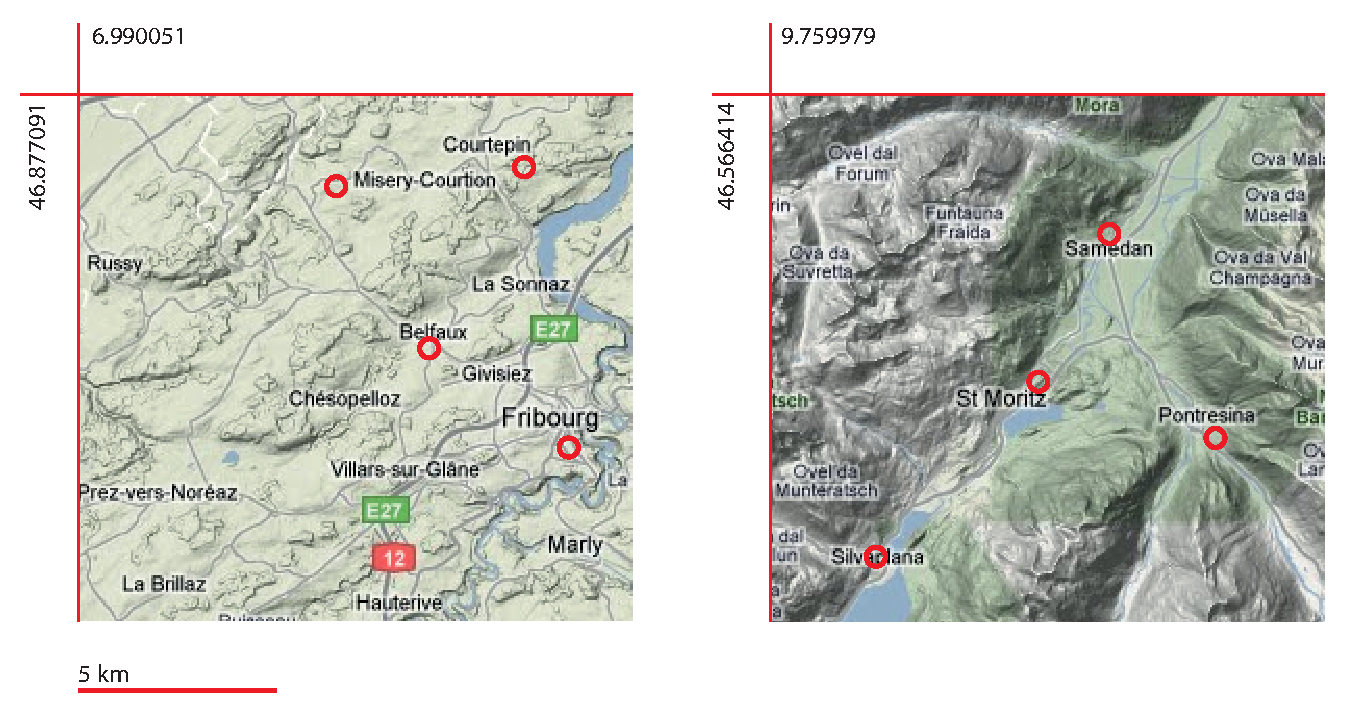
\includegraphics[width=\linewidth]{../figures/site}
	\caption{The two study sites: a relatively flat region around Fribourg and a more mountainous region around St. Moritz. Coordinates are given as latitude/longitude in WGS84.}
	\label{fig:site}
\end{figure}

We expect to find that the smaller roads correspond more closely to results generated by the active walker model, while larger cantonal roads, being further removed from their trail origins, should correspond less with model results. We further expect increasingly mountainous terrain to tightly constrain possible routes: we expect closer correlation between road systems and generated model results in mountainous regions than in the lowlands, since there are less possibilities for taking a route with low associated energy cost.


%=-=-=-=-=-=-=-=-=-=-=-=-=-=-=-=-=-=-=-=-=-=-=-=-=-=-=-=-=-=-=-=-=-=

%=-=-=-=-=-=-=-=-=-=-=-=-=-=-=-=-=-=-=-=-=-=-=-=-=-=-=-=-=-=-=-=-=-=
\section{Description of the Model}
%=-=-=-=-=-=-=-=-=-=-=-=-=-=-=-=-=-=-=-=-=-=-=-=-=-=-=-=-=-=-=-=-=-=

%(Cellular Automata, Agent-Based Model, Continuous Modeling…)
%(If you are not sure here: 1. Consult your colleagues, 2. ask the teachers, 3. remember that you can change it afterwards)
%=-=-=-=-=-=-=-=-=-=-=-=-=-=-=-=-=-=-=-=-=-=-=-=-=-=-=-=-=-=-=-=-=-=
\section{Implementation}
%=-=-=-=-=-=-=-=-=-=-=-=-=-=-=-=-=-=-=-=-=-=-=-=-=-=-=-=-=-=-=-=-=-=

%(What are the answers to the above questions that you expect to find before starting your research?)

%=-=-=-=-=-=-=-=-=-=-=-=-=-=-=-=-=-=-=-=-=-=-=-=-=-=-=-=-=-=-=-=-=-=
\section{Simulation Results and Discussion}
%=-=-=-=-=-=-=-=-=-=-=-=-=-=-=-=-=-=-=-=-=-=-=-=-=-=-=-=-=-=-=-=-=-=
In our analysis of the path formation process using our active walker model, the biggest uncertainty concerned the values of the various independent parameters (durability and intensity of trails, visibility, relative importance of the destination vector). No literature values could be found for these parameters (they are dependent on model specifics such as the model scale). Since our initial hypotheses cannot be conclusively addressed without dealing with the issue of model parameters, we first discuss the effects parameter variation has on model results. We then compare our results with existing road structures.

%=-=-=-=-=-=-=-=-=-=-=-=-=-=-=-=-=-=-=-=-=-=-=-=-=-=-=-=-=-=-=-=-=-=
\subsection{Parameter variation}
A systematic parameter variation study was performed. The two test sites were set up with fixed destinations corresponding to the largest cities in the area. An appropriate range of possible values was chosen for each of the four independent model parameters and the model run for 100 steps for each possible parameter combination. 

\subsubsection{Visibility}
\begin{figure}[tbp]
	\includegraphics[width=\linewidth]{../figures/visibility}
	\caption{The effect of the visibility parameter on attractiveness structure. At low visibilities, the attractiveness reflects the terrain, whereas at high visibilities agents focus more on their destination and terrain details are lost.}
	\label{fig:vis}
\end{figure}
Unfortunately, due to a {\sc matlab} error, the visibility parameter could not be systematically analyzed. The following discussion is therefore of a qualitative nature. As described in \autoref{trail_potential}, visibility controls how fast the influence of an agent's surroundings decreases with distance. As can be seen in \autoref{fig:vis}, a higher visibility causes the attractiveness to ``soften'': the terrain details present at a visibility of 0.3 are lost at a visibility of 4. This causes the agent to consider a larger area in his decision, resulting in a more efficient path taken. Also, paths resulting paths may be more diverse, as different paths have similar efficiency when viewed over a large area rather than simply in the immediate vicinity.

\subsubsection{Importance}
As described in \autoref{pedestrians_direction}, the importance parameter controls how the destination is weighted against an agent's preference for walking in the most attractive direction. A higher importance causes the destination vector to be weighed more heavily, whereas a lower importance causes the attractiveness vector to be weighed more heavily. In \autoref{table:importance1}, the average number of completed paths (agents having reached their destination) after 100 model steps is listed. As might be expected, a higher importance results in significantly more agents reaching their destination. If the importance is lower, agents wander around in the direction where walking is easiest, never reaching their destination (\autoref{fig:importance}). It is difficult, however, to determine what value of importance is the ``correct'' one. Real agents may prefer taking a detour if it means they can walk more comfortably. Also, \autoref{table:importance2} indicates that \emph{when} agents manage to reach their destination, their travel times don't vary considerably. However, all-in-all, since considerably more agents manage to reach their destination within the timespan of 100 model steps when importance is high, this can be considered the more efficient system.

\begin{table}[htbp]
\begin{center}
 \setlength{\abovecaptionskip}{0pt}
 \setlength{\belowcaptionskip}{10pt}
\caption{The average number of completed paths (agents having reached their destination) after 100 model steps as a function of the parameter \emph{importance}.}
\begin{tabular}{r l l l}
  \hline
  \emph{importance} & 0.5 & 1 & 1.6 \\
  \emph{Fribourg} & 3.2 & 23.2 & 88.2  \\ 
  \emph{St. Moritz} & 5.9 & 26.4 & 89.3  \\
\hline
\end{tabular}
\label{table:importance1}
\end{center}
\end{table}

\begin{table}[htbp]
\begin{center}
 \setlength{\abovecaptionskip}{0pt}
 \setlength{\belowcaptionskip}{10pt}
\caption{The average normed travel time (time divided by point-to-point distance) of completed paths after 100 model steps as a function of the parameter \emph{importance}.}
\begin{tabular}{r l l l}
  \hline
  \emph{importance} & 0.5 & 1 & 1.6 \\
  \emph{Fribourg} & 0.15 & 0.22 & 0.16  \\ 
  \emph{St. Moritz} & 0.16 & 0.18 & 0.20  \\
\hline
\end{tabular}
\label{table:importance2}
\end{center}
\end{table}

\begin{figure}[tbp]
	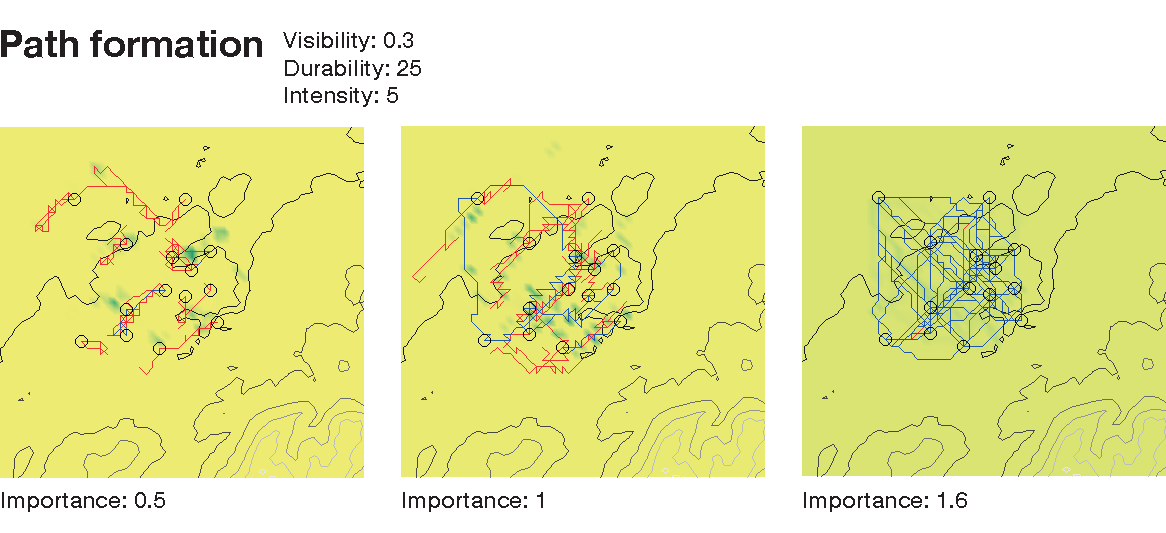
\includegraphics[width=\linewidth]{../figures/importance}
	\caption{Path formation as a function of parameter \emph{importance} at site Fribourg. Blue lines are completed paths, red lines are agents that have not yet reached their destination. The number of agents that reach their destination increases with increasing importance: whereas at an importance of 1.6 many paths are completed, at an importance of 0.5 most agents fail to reach their destination, preferring to wander aimlessly.}
	\label{fig:importance}
\end{figure}


\subsubsection{Durability and Intensity}
The parameters \emph{durability} and \emph{intensity} 

higher clustering, but only at high intensities. more pronounced at fribourg, since st. moritz is constrained anyway.



%=-=-=-=-=-=-=-=-=-=-=-=-=-=-=-=-=-=-=-=-=-=-=-=-=-=-=-=-=-=-=-=-=-=
\subsection{Existing road structure}
\label{sec:roads}

\begin{figure}[tbp]
	\includegraphics[width=\linewidth]{../figures/roads}
	\caption{The road structure at the two study sites (A: Fribourg, B: St. Moritz). Coordinates are given in the reference frame CH1903. The line weight is derived from road class order (highways and 1. order roads are heavier in weight than higher order roads; see \citet{vector25}) and does not necessarily correlate to throughput.}
	\label{fig:roads}
\end{figure}

qualitative differences between the two sites. Road structure at the St. Moritz site shows close similarity to the structure of alpine rivers, 




%=-=-=-=-=-=-=-=-=-=-=-=-=-=-=-=-=-=-=-=-=-=-=-=-=-=-=-=-=-=-=-=-=-=
\section{Summary and Outlook}
%=-=-=-=-=-=-=-=-=-=-=-=-=-=-=-=-=-=-=-=-=-=-=-=-=-=-=-=-=-=-=-=-=-=
We found:
-it's most important to determine correct parameter values
-there are qualitative differences between the two study sites.

%=-=-=-=-=-=-=-=-=-=-=-=-=-=-=-=-=-=-=-=-=-=-=-=-=-=-=-=-=-=-=-=-=-=
%\addcontentsline{toc}{section}{References}  % adds references section to TOC
%\bibliographystyle{apalike2}
%\bibliography{references}

\renewcommand{\refname}{\section{References}} % Using "Sources" as the title of the section
\bibliographystyle{apalike2}
\bibliography{references}


\newpage
%=-=-=-=-=-=-=-=-=-=-=-=-=-=-=-=-=-=-=-=-=-=-=-=-=-=-=-=-=-=-=-=-=-=
\section{Appendix: Matlab Code}
%=-=-=-=-=-=-=-=-=-=-=-=-=-=-=-=-=-=-=-=-=-=-=-=-=-=-=-=-=-=-=-=-=-=
\subsection*{batch.m}
\lstinputlisting{../matlab/batch.m}
\subsection*{Path.m}
\lstinputlisting{../matlab/Path.m}
\subsection*{Pedestrian.m}
\lstinputlisting{../matlab/Pedestrian.m}
\subsection*{Plain.m}
\lstinputlisting{../matlab/Plain.m}
\subsection*{smDriver.m}
\lstinputlisting{../matlab/smDriver.m}
\subsection*{StateMachine.m}
\lstinputlisting{../matlab/StateMachine.m}
\subsection*{visualization.m}
\lstinputlisting{../matlab/visualization.m}


\end{document}
